\section{Evaluation}\label{sec:clf_evaluation}

We evaluate the following sequential selection baselines:

\begin{itemize}
\item \textbf{Static, greedy}: corresponds to best performance of a policy that does not observe feature values and selects actions greedily ($\gamma=0$).
\item \textbf{Static, non-myopic}: policy that does not observe feature values but uses the MDP machinery with $\gamma=1$ to consider future action rewards.
\item \textbf{Dynamic, greedy}: policy that observed feature values, but selects actions greedily.
\end{itemize}

Our method is the \textbf{Dynamic, non-myopic} policy: observed feature values, and full lookahead.

We evaluate two forms of test-time efficient performance measure: the area under the curve and the performance at max budget, although note that all methods are trained only for the former measure.

In preliminary experiments, Logistic Regression always performed better than the Gaussian Naive Bayes classifier, and so only the former is used in the experiments below.
We largely rely on classifier implementations in the \texttt{scikit-learn} package \parencite{Pedregosa2011}.

As described above, we evaluated classification with \textbf{Gaussian} vs. \textbf{Mean} imputation, and with different number of classifiers (1, 3, and 6) clustered by feature subsets.
We found that mean imputation performed better than Gaussian imputation, and although increased number of classifiers sometimes increased performance, it also made our method more prone to overfitting; $K=1$ classifiers worked best on all tasks.
In the following section, we provide detailed results of preliminary evaluation of the imputation method.
After that, we report only the best achieved imputation method.

\subsection{Missing value imputation}\label{sec:clf_eval_imputation}

We evaluate reconstruction and classification error on two datasets: Digits and Scenes-15.
Two feature selection policies are considered: Random and Clustered.
For each policy, we consider Independent and Block-wise selection patterns.

We find that mean imputation with classifier retraining is a reasonably well-performing approach.
Nearest Neighbor methods perform best but are the most expensive.
Gaussian imputation method performs very well, but is also expensive.

Training classifiers with a loss function modified to expect a certain level of feature corruption did not improve performance.
Training additional classifiers for clusters of observed feature subsets did not improve performance.

Feature selection had four experimental conditions.
\begin{itemize}
\item
In \textbf{Random, Independent} selection, each feature was selected independently, and the total number of possible masks for a given budget was not bounded, such that each test instance could have a unique mask (if the number of test instances $N$ was less than the total number of possible feature subsets $2^F$.

\item
In \textbf{Random, Block-wise} selection, there was no bound on the number of possible masks for a given budget, but features were selected by blocks.

\item
In \textbf{Clustered, Independent} selection, each feature was selected independently, but there were at most $K$ possible masks for a given budget.

\item
In \textbf{Clustered, Block-wise} selection, there were at most $K$ possible masks for a budget, and features were selected by blocks.
\end{itemize}

The MCF method is only evaluated in the \textbf{Random, Independent} policy setting, most advantageous to its assumptions.

All datasets were first standardized by subtracting the row mean and dividing by the row standard deviation.

\subsubsection{Digits}
The Digits dataset contains 8x8 grayscale images of hand-written digits 1-10.
Each of the 10 classes has 200 samples, for a total of 2000 images and 64 features.

The dataset was split 60-40 into training and testing sets.
The number of clusters for clustered selection was 10.
For block-wise feature selection, the number of blocks was set to 8.

Figure~\ref{fig:digits} shows the results; here we summarize the conclusions:
\begin{itemize}
\item Mean imputation has highest reconstruction and classification error, aside from SVD, which was so bad that its curves were not plotted.
\item Dot product-based kNN imputation performs worse than Gaussian imputation for both reconstruction and classification, and is slower.
\item Euclidean distance-based kNN imputation performs best, but is slowest.
\item Retraining classifier with mean imputation makes a big difference, while retraining classifier with Gaussian imputation does not make a difference at all.
Presumably, Gaussian imputation maintains the feature statistics of the fully-observed classifier sufficiently well.
\item Modifying the loss function with MCF results in worse performance than doing mean imputation and retraining (MCF evaluated only on the \textbf{Random, Independent} policy).
\item Training additional classifiers for clusters of observed susbets does not make a difference to classification performance.
\item These results hold for all policy experimental conditions.
\end{itemize}

\begin{figure}[ht]
    \centering
    \begin{subfigure}[b]{.9\textwidth}
        \centering
        \includegraphics[width=\linewidth]{../../figures/281b/digits/random_-1/subplots.png}
        \caption{Random, independent feature selection.\vspace{.2cm}}
    \end{subfigure}
    \begin{subfigure}[b]{.9\textwidth}
        \centering
        \includegraphics[width=\linewidth]{../../figures/281b/digits/random_8/subplots.png}
        \caption{Random, block-wise (8 blocks) feature selection.\vspace{.2cm}}
    \end{subfigure}
    \begin{subfigure}[b]{\textwidth}
        \centering
        \includegraphics[width=\linewidth]{../../figures/281b/digits/clustered_-1/subplots.png}
        \caption{Clustered (10 clusters), independent feature selection.\vspace{.2cm}}
    \end{subfigure}
    \begin{subfigure}[b]{\textwidth}
        \centering
        \includegraphics[width=\linewidth]{../../figures/281b/digits/clustered_8/subplots.png}
        \caption{Clustered (10 clusters), block-wise (8 blocks) feature selection.\vspace{.2cm}}
    \end{subfigure}

    \begin{subfigure}[t]{.48\textwidth}
        \centering
        \tiny{\begin{tabular}{ll}
\toprule
                                   & clustered\\
\midrule
gaussian, full                     & 0.206\\
gaussian, retrained                & 0.206\\
kNN (dot)                          & 0.241\\
kNN (dot), full                    & 0.211\\
kNN (euclidean)                    & \textbf{0.166}\\
kNN (euclidean), full              & 0.170\\
mean, full                         & 0.308\\
mean, retrained                    & 0.223\\
mean, retrained, 5 clusters        & 0.301\\
mean, retrained, all (10) clusters & 0.194\\
\bottomrule
\end{tabular}
}
        \caption{Areas under the Classification Error vs. Budget curves. Lower is better.}
    \end{subfigure}\hfill%
    \begin{subfigure}[t]{.48\textwidth}
        \centering
        \tiny{\begin{tabular}{lllll}
\toprule
                & clustered & clustered, blocks & clustered & clustered, blocks\\
\midrule
gaussian        & 94.76     & 93.16             & 151.43    & 150.06\\
kNN (dot)       & 102.5     & 97.59             & 180.11    & 170.79\\
kNN (euclidean) & 87.33     & 87.16             & 159.33    & 159.09\\
mean            & 120.08    & 114.02            & 252.38    & 237.75\\
\bottomrule
\end{tabular}

}
        \caption{Areas under the Reconstruction RMSE vs. Budget curves. Lower is better.}
    \end{subfigure}
    \caption{All results on the \textbf{Digits} dataset.}
    \label{fig:digits}
\end{figure}

\subsubsection{Scenes-15}
The Scene-15 dataset \cite{Lazebnik-CVPR-2006} contains 4485 images from 15 visual scene classes.
The task is to identify classify images according to scene.

Following \cite{Xiao-CVPR-2010}, we extracted 14 different visual features (GIST, HOG, TinyImages, LBP, SIFT, Line Histograms, Self-Similarity, Textons, Color Histograms, and variations).
Separate multi-class linear SVMs were trained on each feature channel, using a random 100 positive example images per class for training.
We used the liblinear implementation, and cross-validated the penalty parameter $C$.

The trained SVMs were evaluated on the images not used for training, resulting in a dataset of 2238 vectors of 210 confidence values: 15 classes for each of the 14 feature channels.
This dataset was split 60-40 into training and test sets for our experiments.
The number of clusters for clustered selection was 10.
For block-wise feature selection, the number of blocks was set to 5.

Figure~\ref{fig:scenes} shows the results.
The conclusions are much the same as for the \textbf{Digits} dataset, with the following additional observations:
\begin{itemize}
\item Gaussian imputation is more costly than kNN on this data; the feature dimensions is more than twice that of the Digits data.
\item For block-wise feature selection, mean imputation with retraining is as good as any other approach, and of course by far the fastest.
\end{itemize}

\begin{figure}[ht]
    \centering
    \begin{subfigure}[b]{.8\textwidth}
        \centering
        \includegraphics[width=\linewidth]{../../figures/281b/scenes/random_-1/subplots.png}
        \caption{Random, independent feature selection.\vspace{.2cm}}
    \end{subfigure}
    \begin{subfigure}[b]{.8\textwidth}
        \centering
        \includegraphics[width=\linewidth]{../../figures/281b/scenes/random_5/subplots.png}
        \caption{Random, block-wise (8 blocks) feature selection.\vspace{.2cm}}
    \end{subfigure}
    \begin{subfigure}[b]{\textwidth}
        \centering
        \includegraphics[width=\linewidth]{../../figures/281b/scenes/clustered_-1/subplots.png}
        \caption{Clustered (10 clusters), independent feature selection.\vspace{.2cm}}
    \end{subfigure}
    \begin{subfigure}[b]{\textwidth}
        \centering
        \includegraphics[width=\linewidth]{../../figures/281b/scenes/clustered_5/subplots.png}
        \caption{Clustered (10 clusters), block-wise (8 blocks) feature selection.\vspace{.2cm}}
    \end{subfigure}

    \begin{subfigure}[b]{1\textwidth}
        \centering
        \tiny{\begin{tabular}{ll}
\toprule
                                   & clustered\\
\midrule
gaussian, full                     & 0.206\\
gaussian, retrained                & 0.206\\
kNN (dot)                          & 0.241\\
kNN (dot), full                    & 0.211\\
kNN (euclidean)                    & \textbf{0.166}\\
kNN (euclidean), full              & 0.170\\
mean, full                         & 0.308\\
mean, retrained                    & 0.223\\
mean, retrained, 5 clusters        & 0.301\\
mean, retrained, all (10) clusters & 0.194\\
\bottomrule
\end{tabular}
}
        \caption{Areas under the Classification Error vs. Budget curves. Lower is better.}
    \end{subfigure}
    \begin{subfigure}[b]{1\textwidth}
        \centering
        \tiny{\begin{tabular}{lllll}
\toprule
                & clustered & clustered, blocks & clustered & clustered, blocks\\
\midrule
gaussian        & 94.76     & 93.16             & 151.43    & 150.06\\
kNN (dot)       & 102.5     & 97.59             & 180.11    & 170.79\\
kNN (euclidean) & 87.33     & 87.16             & 159.33    & 159.09\\
mean            & 120.08    & 114.02            & 252.38    & 237.75\\
\bottomrule
\end{tabular}

}
        \caption{Areas under the Reconstruction RMSE vs. Budget curves. Lower is better.}
    \end{subfigure}
    \caption{All results on the \textbf{Scenes-15} dataset.}
    \label{fig:scenes}
\end{figure}

\subsubsection{Conclusion}

On both datasets, and for all feature selection approaches, we find that mean imputation (with a classifier trained on imputed data) is a well-performing approach.
Nearest Neighbor and Gaussian methods perform best but are the most expensive; Gaussian scales poorly with number of features, while NN scales poorly with size of training set.

We did not find that using Marginalized Corrupted Features loss function improved classification performance.
In fact, the simple baseline approach of mean imputation with classifier retraining performed better.
Training additional classifiers for clusters of observed feature subsets also did not improve performance on these datasets.
Further study of this method is needed.


\subsection{Experiment: Synthetic}

\begin{figure*}[ht]
\centering
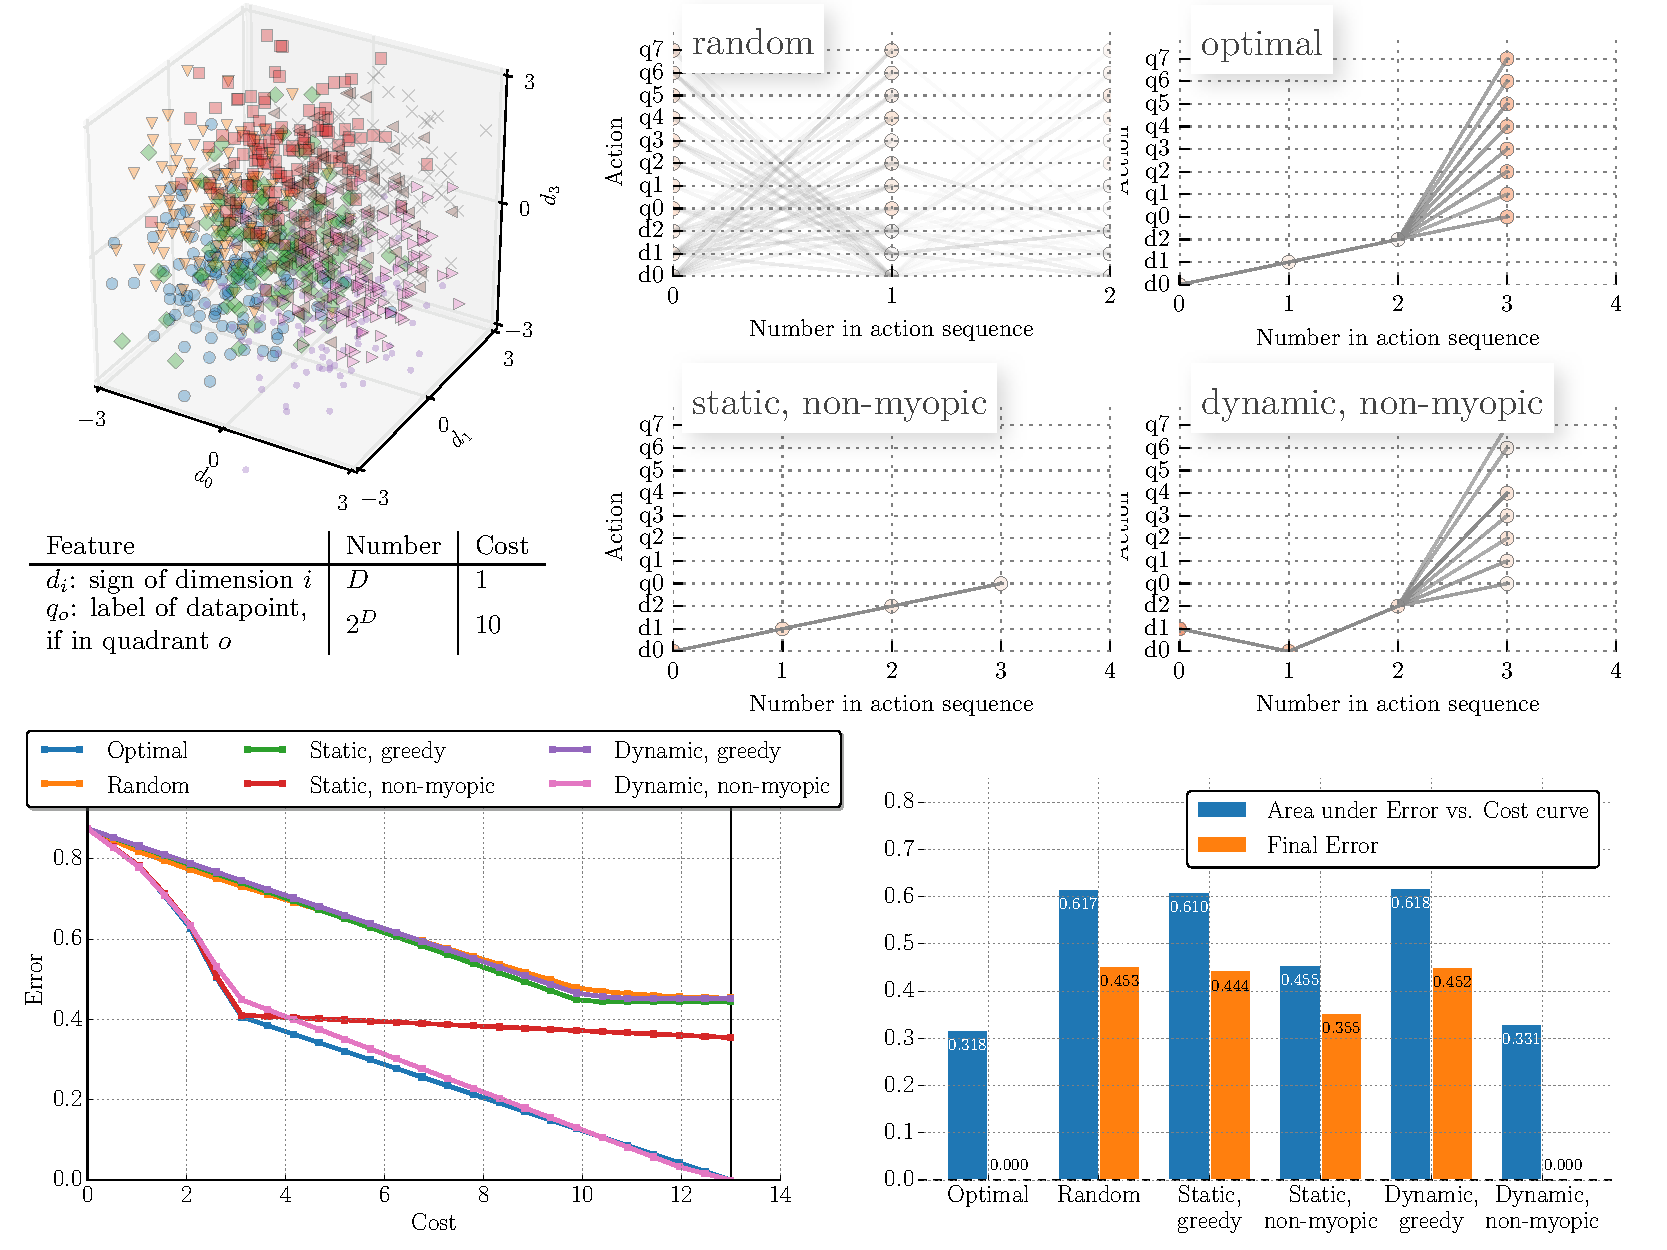
\includegraphics[width=\linewidth]{../../figures/synthetic.pdf}
\caption{
Evaluation on the synthetic example (best viewed in color).
The data and the feature costs are shown at top left; the sample feature trajectories of different policies at top right.
(The opacity of the edges corresponds to their prevalence during policy execution; the opacity of the nodes corresponds to the amount of reward obtained in that state.)
Note that the \emph{static, non-myopic} policy correctly learns to select the cheap features first, but is not able to correctly branch, while our \emph{dynamic, non-myopic} approach finds the optimal strategy.
The plots in the bottom half give the error vs. cost numbers.
}\label{fig:synthetic}
\end{figure*}


Following \parencite{Xu-ICML-2013}, we first show that the policy works as advertised in a challenging synthetic example.
In $D$-dimensional space, the data has a label for each of the $2^D$ orthants, and is generated by a unit-variance Gaussian in that orthant (See top left of \autoref{fig:synthetic} for the 3D case).
There are $D$ cheap features that simply return the sign of the data point's coordinate for the corresponding dimension.
For each orthant, there is also an expensive feature that returns the data point's label if the point is located in the corresponding orthant, and random noise otherwise.

The optimal policy on a new data point is to determine its orthant with cheap features, and then take the corresponding expensive action.
Note that both dynamic features and non-myopic learning are crucial to the optimal policy, which is successfully found by our approach.
\autoref{fig:synthetic} shows the results of this optimal policy, a random policy, and of different baselines and our method, trained given the correct minimal budget.

\subsection{Experiment: Scene recognition}

%!TEX root=paper/paper.tex
\begin{figure*}[ht]
\centering
    \centering
    \begin{subfigure}[b]{0.5\textwidth}
            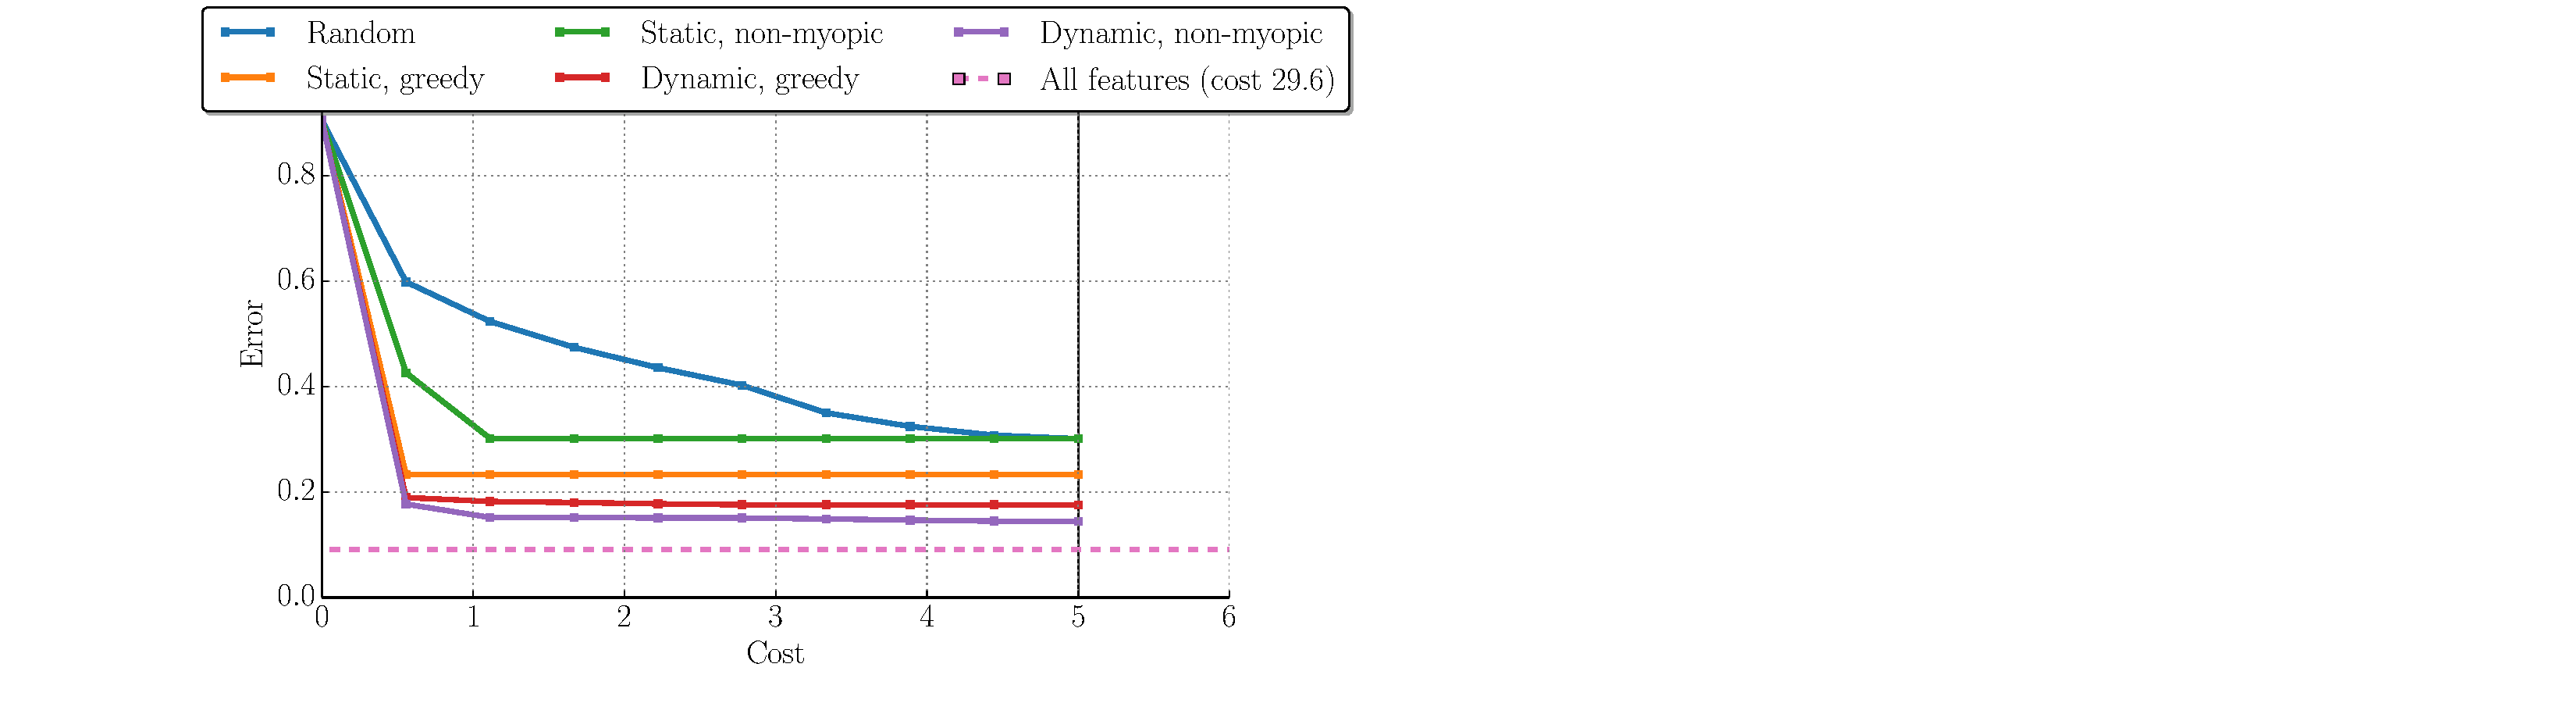
\includegraphics[width=\textwidth]{../../figures/apr11_assembly/scene_15_5_crop.pdf}
            \caption{Error given by policies learned for a budget = 5.}
    \end{subfigure}%
    \begin{subfigure}[b]{0.44\textwidth}
            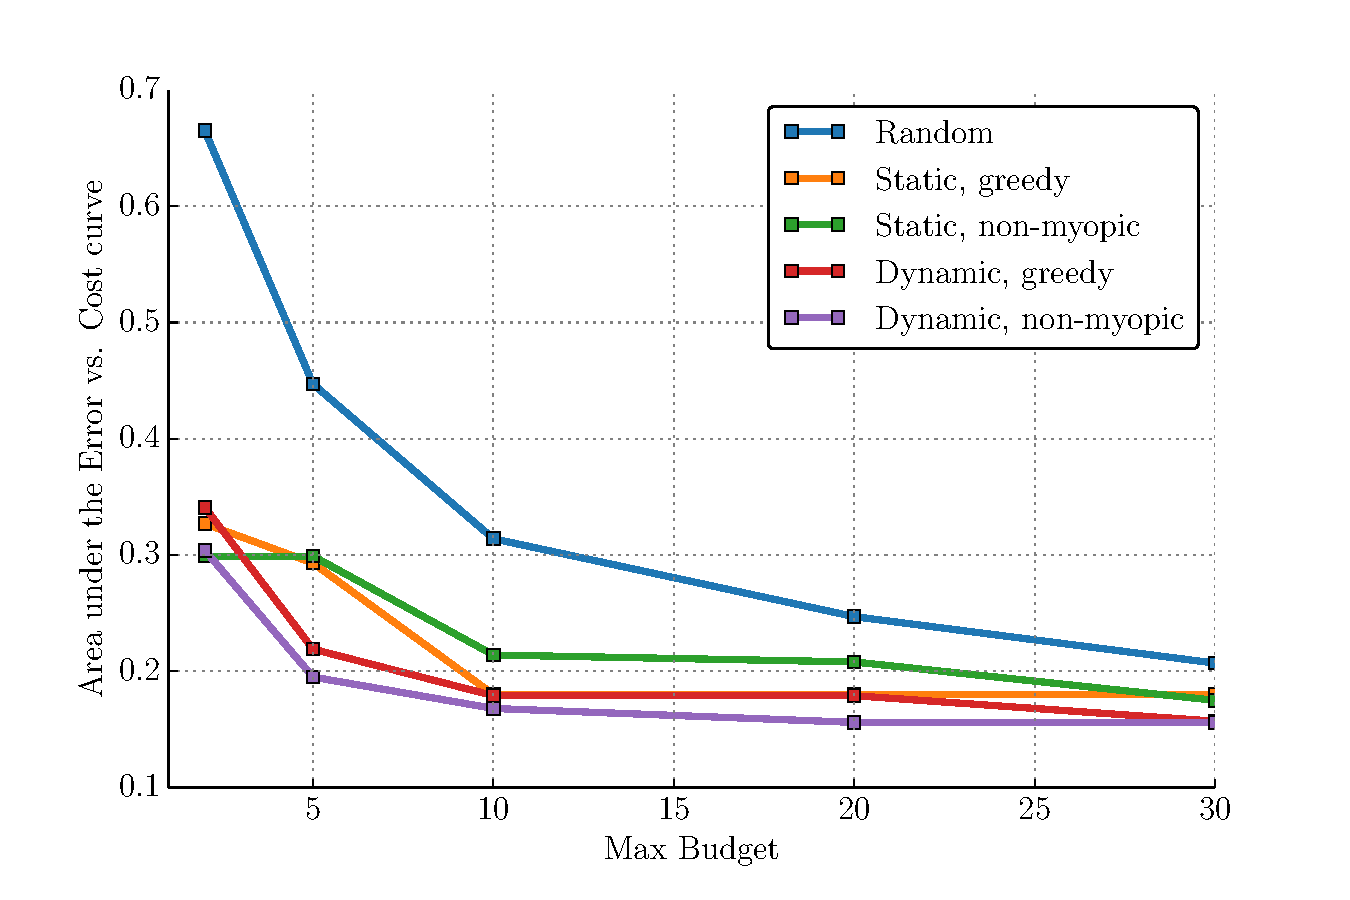
\includegraphics[width=\textwidth]{../../figures/apr11_assembly/_scenes15_auc.pdf}
            \caption{Areas under error vs. cost curves of policies learned at different budgets.}
    \end{subfigure}\\
    \begin{subfigure}[b]{0.47\textwidth}
            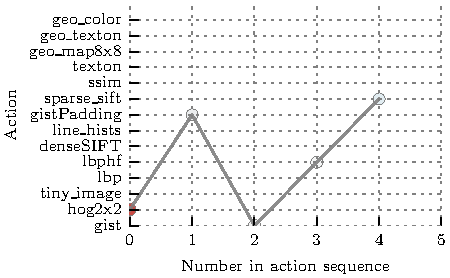
\includegraphics[width=\textwidth]{../../figures/apr11_assembly/scene15_5/static.pdf}
            \caption{Trajectory of our static policy.}
    \end{subfigure}%
    \begin{subfigure}[b]{0.47\textwidth}
            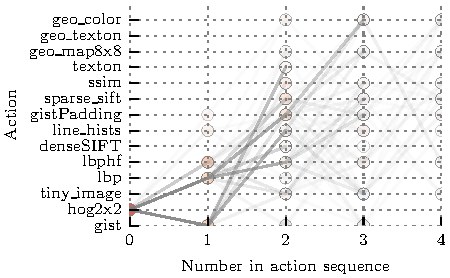
\includegraphics[width=\textwidth]{../../figures/apr11_assembly/scene15_5/dynamic.pdf}
            \caption{Trajectory of our dynamic policy.}
    \end{subfigure}\\
    \caption[Results of the classification approach on the Scenes-15 dataset.]{
Results on Scenes-15 dataset (best viewed in color).
Figure (a) shows the error vs. cost plot for policies learned given a budget of 5 seconds.
Figure (b) aggregates the area under the error vs. cost plot metrics for different policies and budgets, showeing that our approach outperforms baselines no matter what budget it's trained for.
Figures (d) and (e) shows the branching behavior of our dynamic policy vs the best static policy.
}\label{fig:clf_scenes}
\end{figure*}


The Scene-15 dataset \parencite{Lazebnik-CVPR-2006} contains 4485 images from 15 visual scene classes.
The task is to classify images according to scene.
Following \parencite{Xiao-CVPR-2010}, we extracted 14 different visual features (GIST, HOG, TinyImages, LBP, SIFT, Line Histograms, Self-Similarity, Textons, Color Histograms, and variations).
The features vary in cost from 0.3 seconds to 8 seconds, and in single-feature accuracy from 0.32 (TinyImages) to .82 (HOG).
Separate multi-class linear SVMs were trained on each feature channel, using a random 100 positive example images per class for training.
We used the \texttt{liblinear} implementation, and K-fold cross-validated the penalty parameter $C$.
The trained SVMs were evaluated on the images not used for training, resulting in a dataset of 2238 vectors of 210 confidence values: 15 classes for each of the 14 feature channels.
This dataset was split 60-40 into training and test sets for our experiments.

\hyperref[fig:scenes]{Figure~\ref*{fig:scenes}} shows the results, including learned policy trajectories.
For all evaluated budgets, our \emph{dynamic, non-myopic} method outperforms all others on the area under the error vs. cost curve metric.
Our results on this dataset match the reported results of Active Classification \parencite{Gao-NIPS-2011} (Figure 2) and Greedy Miser \parencite{Xu-ICML-2012} (Figure 3), although both methods use an additional powerful feature channel (ObjectBank)\footnote{Detailed results for this and other experiments are on the project page (see front page for the \href{http://sergeykarayev.com/recognition-on-a-budget/}{link}).}.

\subsection{Experiment: ImageNet and maximizing specificity}

\begin{figure*}[ht]
\centering
    \begin{subfigure}[b]{0.52\textwidth}
            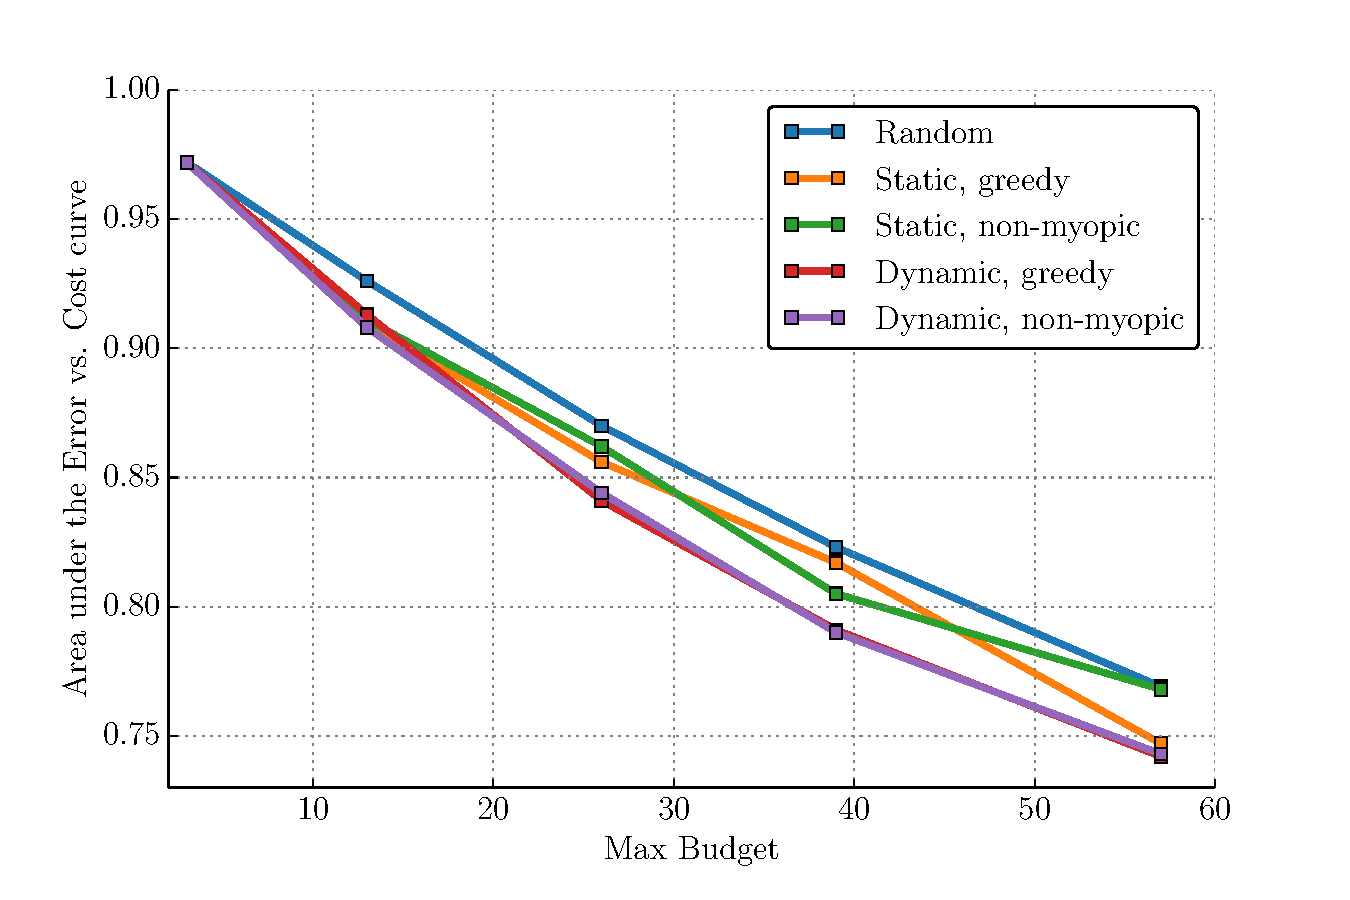
\includegraphics[width=\textwidth]{../../figures/apr11_assembly/_ilsvrc65_auc.pdf}
            \caption{
            Areas under error vs. cost curves for policies learned at different budgets.
            (No specificity back-off is performed here).
            \label{fig:imagenet-a}
            }
    \end{subfigure}\hfill%
    \begin{subfigure}[b]{0.43\textwidth}
            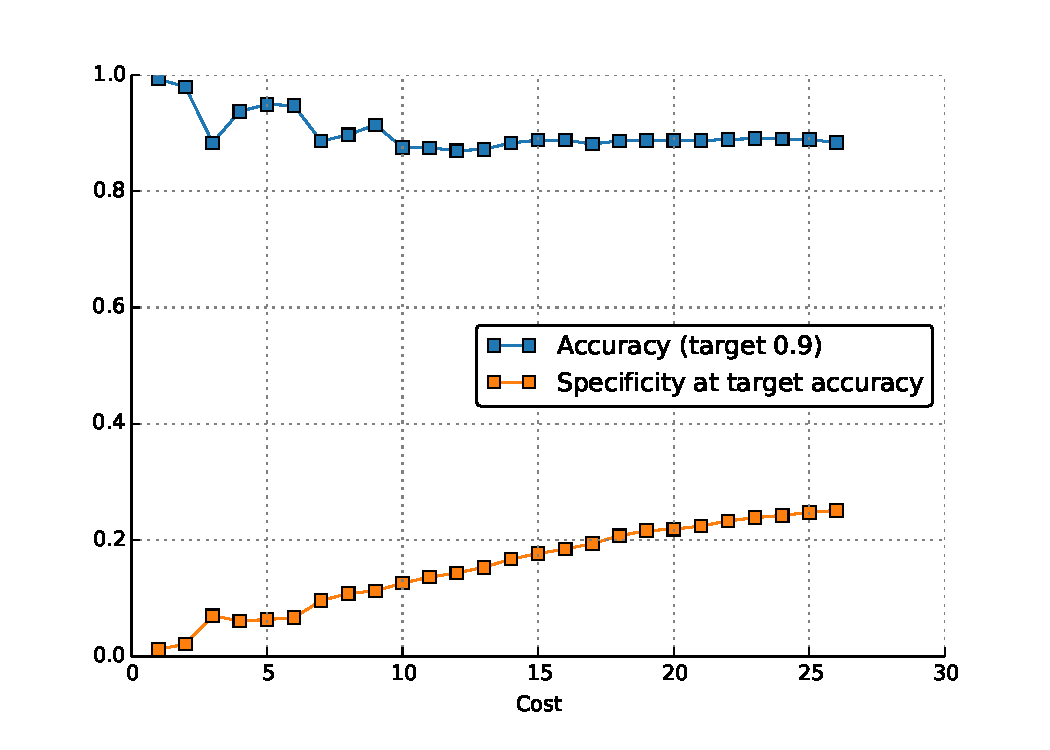
\includegraphics[width=\textwidth]{../../figures/apr11_assembly/ilsvrc65_acc.pdf}
            \caption{
            Holding prediction accuracy constant, we achieve increased specificity with increased cost (on \emph{Dynamic, non-myopic} policy, budget = 36).
            \label{fig:imagenet-b}
            }
    \end{subfigure}\\\vspace{1em}
    \begin{subfigure}[b]{.97\textwidth}
            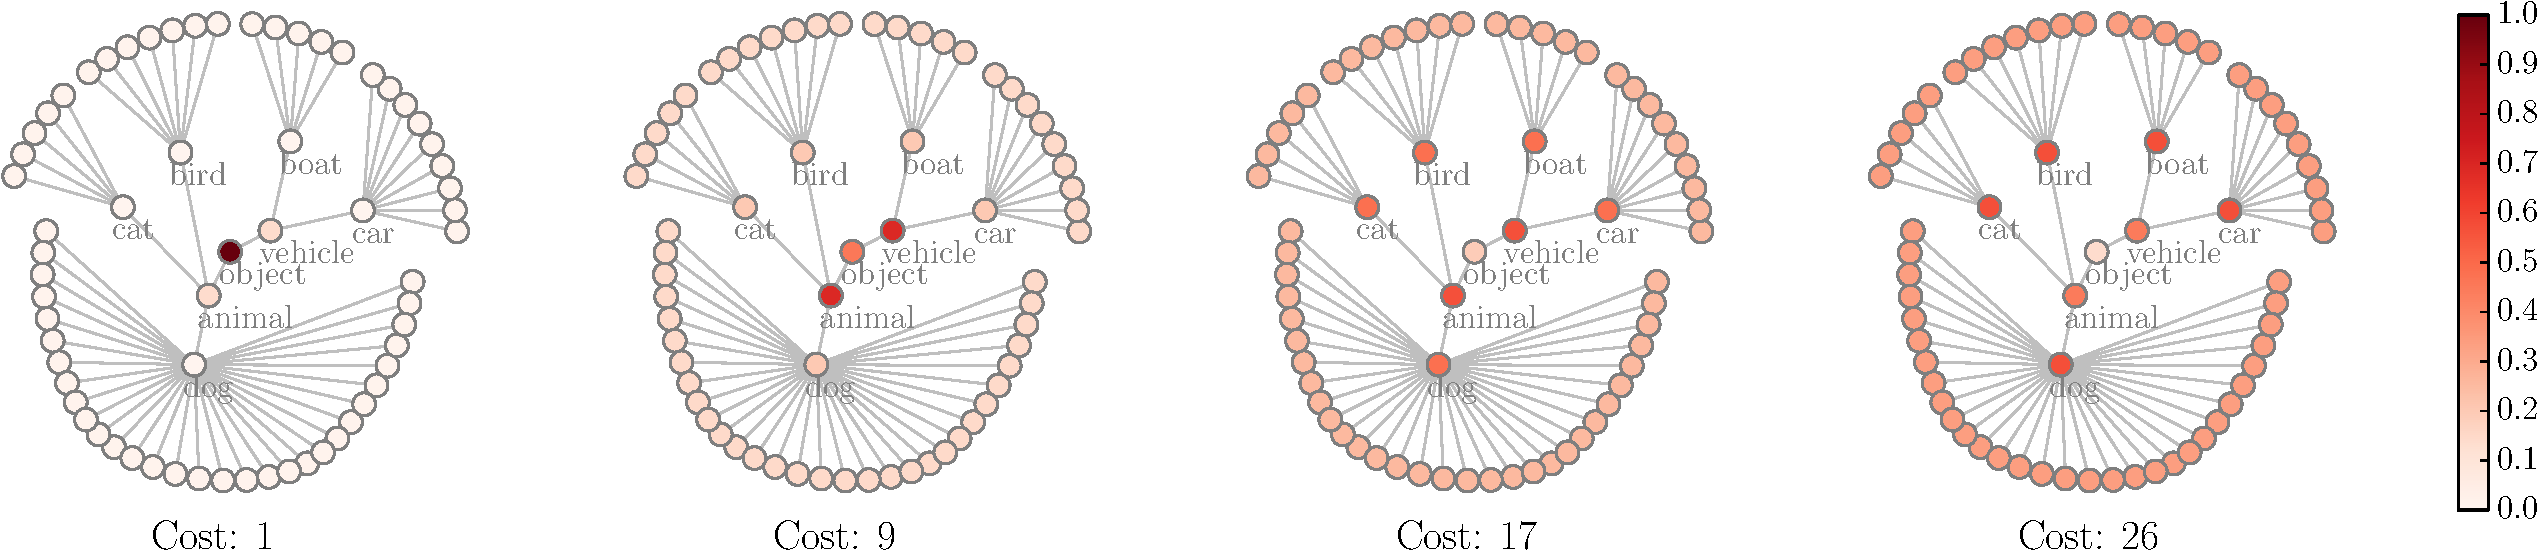
\includegraphics[width=\textwidth]{../../figures/apr11_assembly/ilsvrc65_network-crop.pdf}
            \caption{
            We visualize the fraction of predictions made at inner vs. leaf nodes of ILSVRC-65 at different cost points of an Anytime policy: with more computation, accurate predictions are increasingly made at the leaf nodes.
            \label{fig:imagenet-c}
            }
    \end{subfigure}
\caption{
Results on the ILSVRC-65 dataset (best viewed in color).
Figure (a) shows our dynamic approaches outperforming static baselines for all practical cost budgets.
When our method is combined with Hedging Your Bets \parencite{Deng-CVPR-2012}, a constant prediction accuracy can be achieved at all points in the Anytime policy, with \emph{specificity} of predictions increasing with the cost of predictions.
Figures (b) and (c) show this for the \emph{dynamic, non-myopic} policy learned for budget = 26.
This is analogous to human visual performance, which shows increased specificity at longer stimulus times.
}\label{fig:imagenet}
\end{figure*}


The full ImageNet dataset has over 10K categories and over a million images \parencite{Deng-ECCV-2010}.
The classes are organized in a hierarchical structure, which can be exploited for novel recognition tasks.
We evaluate on a 65-class subset introduced in ``Hedging Your Bets'' \parencite{Deng-CVPR-2012}.
In this evaluation, we consider the situation where the initial feature computation has already happened, and the task is to find a path through existing one-vs-all classifiers: features correspond to Platt-scaled SVM confidences of leaf-node classifiers (trained on SIFT-LLC features), and each has cost 1 \parencite{Deng-ECCV-2010}.
Following \parencite{Deng-CVPR-2012}, accuracy is defined on all nodes, and inner node confidences are obtained by summing the probabilities of the descendant nodes.

We combine our sequential feature selection with the ``Hedging Your Bets'' method for backing off prediction nodes using the ImageNet hierarchy to maintain guaranteed accuracy while giving maximally specific answers, given a cost budget.
The results are given in \hyperref[fig:imagenet]{Figure~\ref*{fig:imagenet}}.
As the available budget increases, the \emph{specificity} (defined by normalized information gain in the hierarchy) of our predictions also increases, while accuracy remains constant.
Visualizing this on the ILSVRC-65 hierarchy, we see that the fraction of predictions at the leaf nodes grows with available computation time.
This formulation presents a novel angle on modeling the time course of human visual perception.
